%%%%%%%%%%%%%%%%%%%%%%%%%%%%%%%%%%%%

\section{標本抽出の原則と方法}

%%%%%%%%%%%%%%%%%%%%%%%%%%%%%%%%%%%%

\subsection{母集団と標本}

%%%%%%%%%%%%%%%%%%%%%%%%%%%%%%%%%%%%

\begin{frame}
\frametitle{母集団と標本}

\twocol{0.5}{0.5}{
\begin{center}
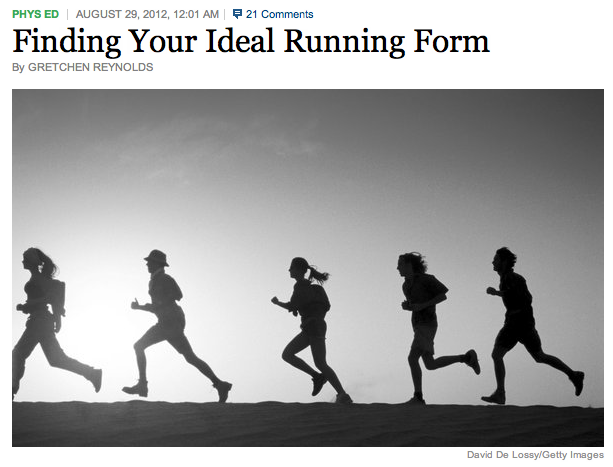
\includegraphics[width=\textwidth]{1-3_sampling_principles_strategies/figures/running}
\end{center}
\vspace{-0.5cm}
{\tiny \webURL{http://well.blogs.nytimes.com/2012/08/29/finding-your-ideal-running-form}}
}
{
\hl{研究の問い：}走ることだけで、より効率的なランナーになれるか？\\

\hl{対象母集団：}\soln{すべての人}
}
$\:$ \\
\hl{標本：}最近ランニンググループに参加した成人女性のグループ

\hl{結果を一般化できる母集団：}\soln{データがランダムにサンプリングされていれば成人女性}

\end{frame}

%%%%%%%%%%%%%%%%%%%%%%%%%%%%%%%%%%%%

\subsection{逸話的証拠}

%%%%%%%%%%%%%%%%%%%%%%%%%%%%%%%%%%%%

\begin{frame}
\frametitle{逸話的証拠と喫煙研究の黎明期}

\begin{itemize}

\item 禁煙研究は1930〜40年代、タバコの喫煙が急増した頃に始まった。
タバコの煙に敏感な喫煙者がいる一方、まったく影響を受けないように見える喫煙者もいた。

\item 禁煙研究は「私の叔父は一日3箱吸っているが至って健康だ」というような
\hl{逸話的証拠}（限られた標本に基づく根拠で、母集団を代表しない可能性がある）
に基づく反論に直面した。

\item 「喫煙は複雑な人間行動であり、その性質上研究しにくく、
個人差によって交絡されている」という結論が出された。

\item やがて研究者たちがより大きな標本（喫煙者）を検討できるようになると、
喫煙が健康に悪影響を及ぼすという傾向がはっきりと見えるようになった。

\end{itemize}

\ct{Brandt, \textit{The Cigarette Century} (2009), Basic Books.}

\end{frame}

%%%%%%%%%%%%%%%%%%%%%%%%%%%%%%%%%%%%

\subsection{母集団からの標本抽出}

%%%%%%%%%%%%%%%%%%%%%%%%%%%%%%%%%%%%

\begin{frame}
\frametitle{全数調査}

\begin{itemize}

\item 全員を対象にして、母集団全体を「サンプリング」した方がよいのではないか？
\begin{itemize}
\item これを\hl{全数調査}という。
\end{itemize}

\item 全数調査には以下のような問題がある：

\begin{itemize}
\item 全員を調査するのは難しい：見つけにくい個人や測定しにくい個人は常に存在する。
\textit{しかも、そのような見つけにくい人々は、他の人々と異なる特性を持っている可能性がある。}
\item 母集団は変化し続ける。全数調査ができたとしても、
母集団は常に変化するため、完全な測定は不可能である。
\item 全数調査は標本抽出より複雑になる場合がある。
\end{itemize}

\end{itemize}

\end{frame}

%%%%%%%%%%%%%%%%%%%%%%%%%%%%%%%%%%%%%

\begin{frame}

\vfill

\begin{center}
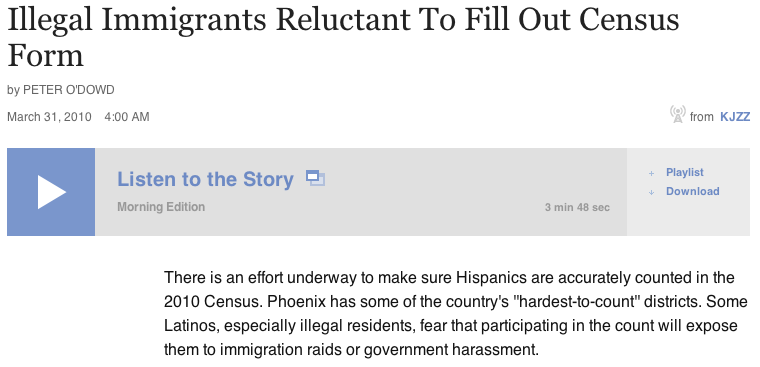
\includegraphics[width=0.90\textwidth]{1-3_sampling_principles_strategies/figures/census_illegal_immig}
\end{center}

\ct{\webURL{http://www.npr.org/templates/story/story.php?storyId=125380052}}

\end{frame}

%%%%%%%%%%%%%%%%%%%%%%%%%%%%%%%%%%%%%

\begin{frame}
\frametitle{探索的分析から推測へ}

\begin{itemize}

\item 標本抽出は自然な営みである。

\item 料理中の食べ物を味見することを考えてみよう――料理全体の味を知るために、
その一部（標本）を味見（検査）する。

\item スープを一口味見して「塩気が足りない」と思うのが\hl{探索的分析}である。

\item そこから「スープ全体に塩が足りない」と結論づけるのが\hl{推測}である。

\item 推測が有効であるためには、味見した一口（標本）が鍋全体（母集団）を
\hl{代表している}必要がある。

\begin{itemize}
\item 表面からしか取っていない一口が、塩が底に溜まっているスープを代表しているとは言えない。
\item よくかき混ぜてから味見すれば、一口はスープ全体を代表しやすくなる。
\end{itemize}

\end{itemize}

\end{frame}

%%%%%%%%%%%%%%%%%%%%%%%%%%%%%%%%%%%%

\begin{frame}
\frametitle{標本バイアス}

\begin{itemize}

\item \hl{無回答バイアス：}ランダムにサンプリングされた人のうちごく一部しか
調査に回答しない場合、標本はもはや母集団を代表していない可能性がある。

\item \hl{自発的回答バイアス：}その問題について強い意見を持つ人が
自ら進んで回答することで標本が構成される場合。
このような標本も母集団を代表しない。

\begin{center}
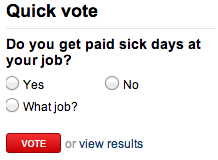
\includegraphics[width=0.25\textwidth]{1-3_sampling_principles_strategies/figures/vol_resp_bias/vol_resp_bias_q}
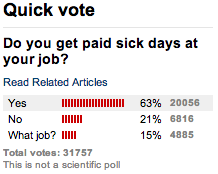
\includegraphics[width=0.25\textwidth]{1-3_sampling_principles_strategies/figures/vol_resp_bias/vol_resp_bias_res} \\
{\tiny cnn.com, 2012年1月14日}
\end{center}

\item \hl{便宜的標本：}アクセスしやすい個人が標本に含まれやすくなる。

\end{itemize}

\end{frame}

%%%%%%%%%%%%%%%%%%%%%%%%%%%%%%%%%%%%

\begin{frame}
\frametitle{標本バイアスの例：ランドン対FDR}

偏った標本が誤った結果をもたらした歴史的な例：\\

$\:$ \\

\begin{columns}[c]

\column{0.35\textwidth}

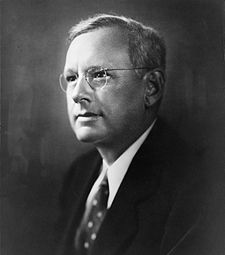
\includegraphics[width= \textwidth]{1-3_sampling_principles_strategies/figures/landon_fdr/landon}

\column{0.3\textwidth}
1936年、ランドンはFDR（フランクリン・ルーズベルト）の再選に対抗して
共和党の大統領候補を目指した。

\column{0.35\textwidth}

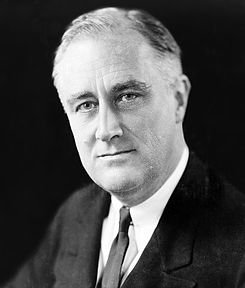
\includegraphics[width= \textwidth]{1-3_sampling_principles_strategies/figures/landon_fdr/fdr}

\end{columns}

\end{frame}

%%%%%%%%%%%%%%%%%%%%%%%%%%%%%%%%%%%%%

\begin{frame}
\frametitle{リテラリー・ダイジェスト誌の世論調査}

\begin{columns}

\column{0.7\textwidth}

\begin{itemize}

\item リテラリー・ダイジェスト誌は約1,000万人のアメリカ人に調査を行い、
約240万人から回答を得た。

\item 調査ではランドンが圧勝し、FDRの得票率は43\%にとどまると予測された。

\item 実際の選挙結果：FDRが62\%の票を獲得して勝利した。

\end{itemize}

\column{0.3\textwidth}

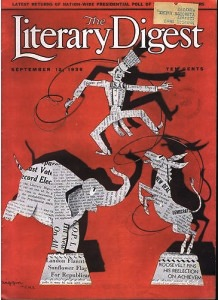
\includegraphics[width= \textwidth]{1-3_sampling_principles_strategies/figures/literaryDigest}

\end{columns}

\begin{itemize}

\item この雑誌は世論調査の失敗によって信頼を完全に失い、まもなく廃刊となった。

\end{itemize}

\end{frame}

%%%%%%%%%%%%%%%%%%%%%%%%%%%%%%%%%%%%%

\begin{frame}
\frametitle{リテラリー・ダイジェスト誌の世論調査――何が間違っていたか？}

\begin{itemize}

\item この雑誌が調査対象としたのは、

\begin{itemize}

\item 自誌の読者、

\item 自動車の登録者、そして

\item 電話の契約者であった。

\end{itemize}

\item これらのグループは当時（大恐慌の時代であることを思い出してほしい）の
全国平均を大きく上回る収入を持っており、
共和党を支持する有権者が多く含まれていた。
つまり標本は当時のアメリカの\hl{典型的な}有権者を代表していなかった。

\end{itemize}

\end{frame}

%%%%%%%%%%%%%%%%%%%%%%%%%%%%%%%%%%%%%

\begin{frame}
\frametitle{大きな標本は望ましいが……}

\begin{itemize}

\item リテラリー・ダイジェスト誌の世論調査は240万人という巨大な標本に基づいていたが、
標本に\hl{バイアス}があったため、正確な予測はできなかった。

\item スープの例えに戻ると：
スープがよくかき混ぜられていなければ、スプーンがいくら大きくても味は正しく分からない。
よくかき混ぜてあれば、小さなスプーンで十分である。

\end{itemize}

\end{frame}

%%%%%%%%%%%%%%%%%%%%%%%%%%%%%%%%%%%%%

\begin{frame}[shrink]
\frametitle{練習問題}

{\small
\pq{ある学区が、最近2件の生徒の重傷事故を受けて、高校生の校内駐車を禁止するか
検討している。最初の一歩として、保護者に郵送でアンケートを行い、
この方針変更に反対するかどうかを尋ねた。送付した6,000通のうち、
返送されたのは1,200通であった。回答のあった1,200通のうち、960通が方針変更に賛成、
240通が反対であった。次の記述のうち正しいものはどれか？}

\begin{enumerate}[I.]
\item 郵便物が保護者に届かなかった可能性がある。
\item 学区は方針変更について保護者から強い支持を得ている。
\item 高校生の保護者の多数が方針変更に反対している可能性がある。
\item すべての保護者に調査票を送ったのだから、調査結果にバイアスが生じる可能性は低い。
\end{enumerate}

\begin{multicols}{5}
\begin{enumerate}[(a)]
\item Iのみ
\item IとII
\solnMult{IとIII}
\item IIIとIV
\item IVのみ
\end{enumerate}
\end{multicols}
}

\end{frame}

%%%%%%%%%%%%%%%%%%%%%%%%%%%%%%%%%%%%%

\subsection{観察研究}

%%%%%%%%%%%%%%%%%%%%%%%%%%%%%%%%%%%%%

\begin{frame}
\frametitle{観察研究}

\begin{itemize}

\item 研究者はデータが生じる過程に直接介入しない方法でデータを収集する。

\item 観察研究の結果は、説明変数と応答変数の間の関連を示すために使えるが、
因果関係を確立することは一般的にできない。

\end{itemize}

\end{frame}

%%%%%%%%%%%%%%%%%%%%%%%%%%%%%%%%%%%%%

\subsection{4つの標本抽出法}

%%%%%%%%%%%%%%%%%%%%%%%%%%%%%%%%%%%%%

\begin{frame}
\frametitle{良い標本の取り方}

\begin{itemize}

\item ほぼすべての統計的手法は、暗黙の無作為性という概念に基づいている。

\item 観察データが母集団からランダムな枠組みで収集されていない場合、
これらの統計的手法――推定値やその誤差――は信頼できない。

\item 最もよく使われる無作為抽出法は、
\hl{単純無作為抽出}、\hl{層化抽出}、\hl{クラスター抽出}である。

\end{itemize}

\end{frame}

%%%%%%%%%%%%%%%%%%%%%%%%%%%%%%%%%%%%

\begin{frame}
\frametitle{単純無作為抽出}

母集団から、選ばれた点同士に関係性がないようにケースをランダムに選択する。

\begin{center}
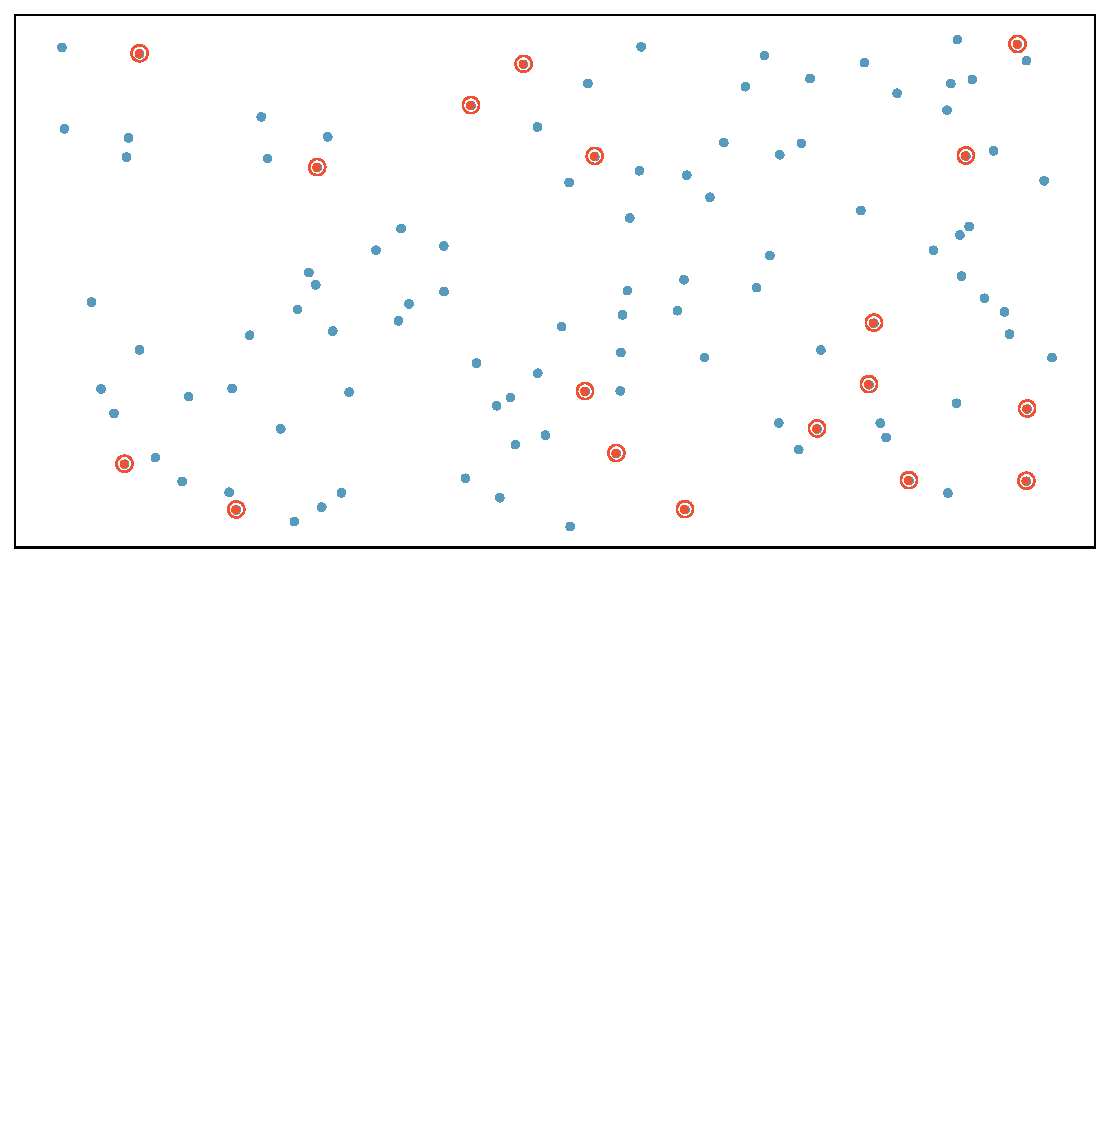
\includegraphics[width=0.9\textwidth]{1-3_sampling_principles_strategies/figures/sampling_methods/simple}
\end{center}

\end{frame}

%%%%%%%%%%%%%%%%%%%%%%%%%%%%%%%%%%%%

\begin{frame}
\frametitle{層化抽出}

\hl{層}は似た観測値からなる。各層から\underline{それぞれ}単純無作為抽出を行う。

\begin{center}
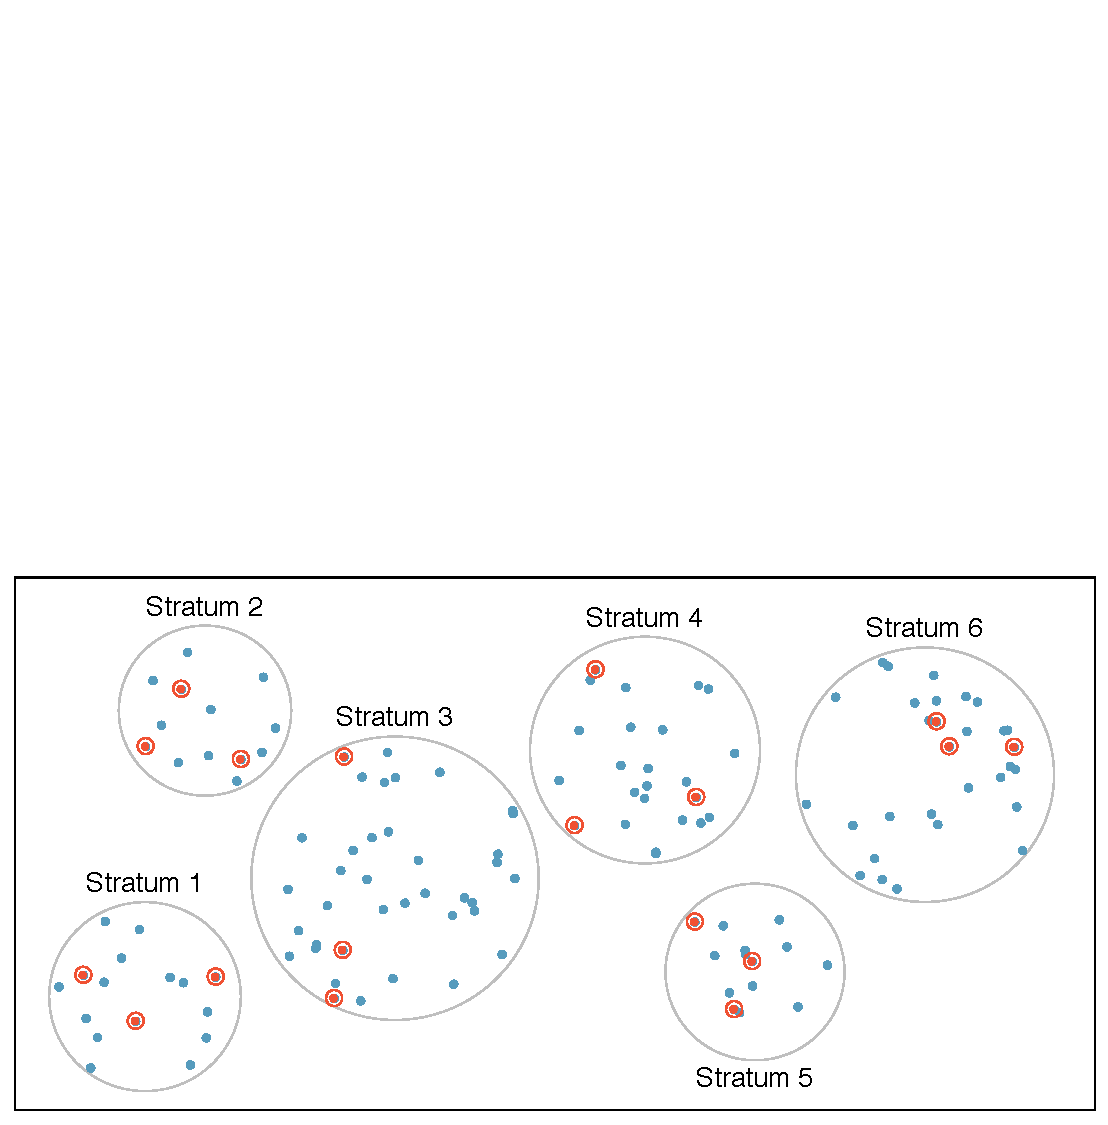
\includegraphics[width=0.9\textwidth]{1-3_sampling_principles_strategies/figures/sampling_methods/stratified}
\end{center}

\end{frame}

%%%%%%%%%%%%%%%%%%%%%%%%%%%%%%%%%%%%

\begin{frame}
\frametitle{クラスター抽出}

\hl{クラスター}は通常、均質な観測値からなるわけではない。
クラスターを単純無作為抽出し、そのクラスター内の\underline{すべて}の観測値を調査する。
経済的な理由から選ばれることが多い。

\begin{center}
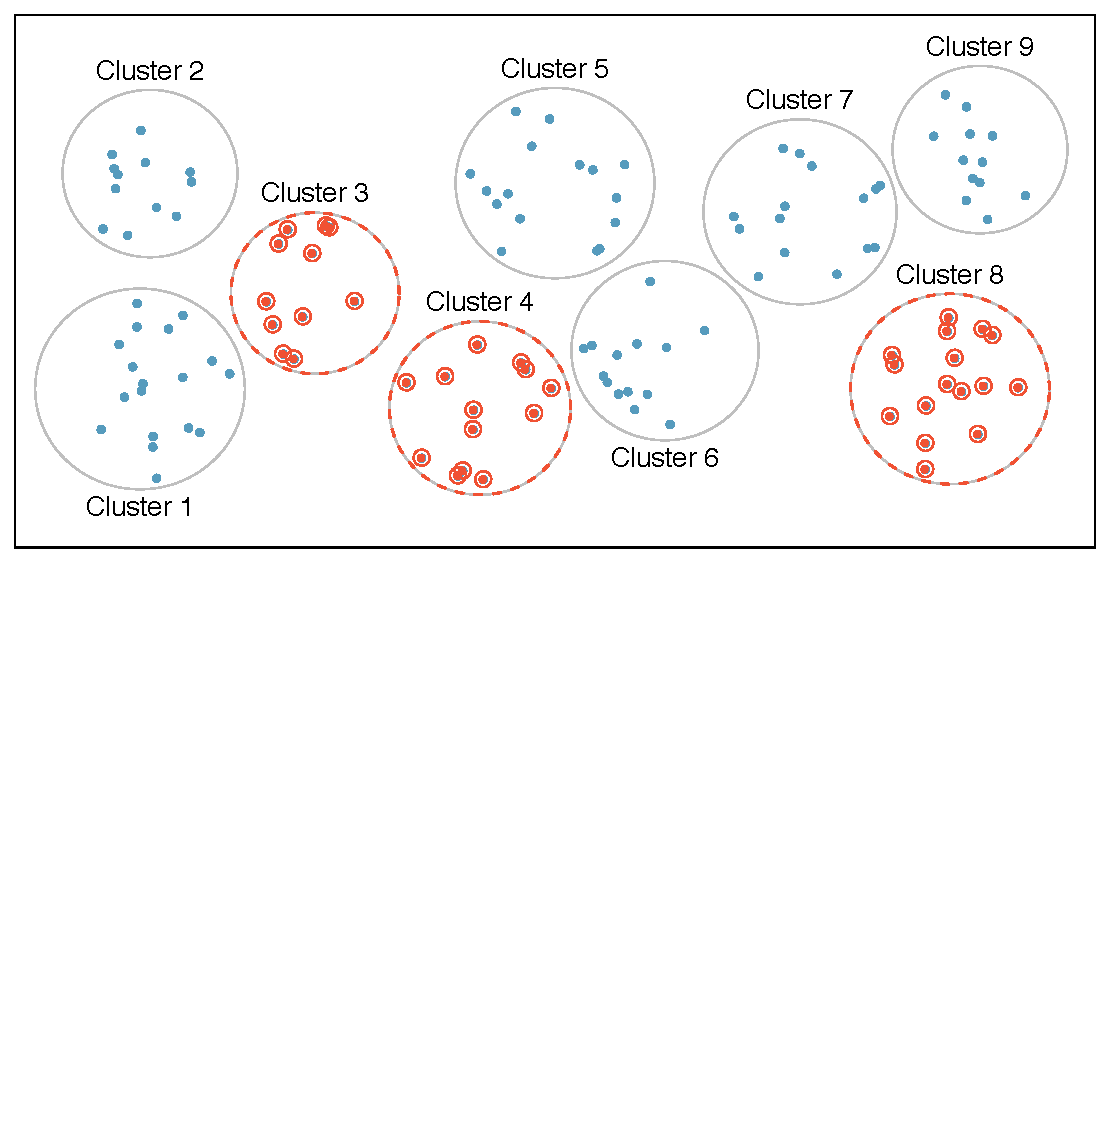
\includegraphics[width=0.9\textwidth]{1-3_sampling_principles_strategies/figures/sampling_methods/cluster}
\end{center}

\end{frame}

%%%%%%%%%%%%%%%%%%%%%%%%%%%%%%%%%%%%

\begin{frame}
\frametitle{多段抽出}

\hl{クラスター}は通常、均質な観測値からなるわけではない。
クラスターを単純無作為抽出し、さらに抽出されたクラスターから観測値を単純無作為抽出する。

\begin{center}
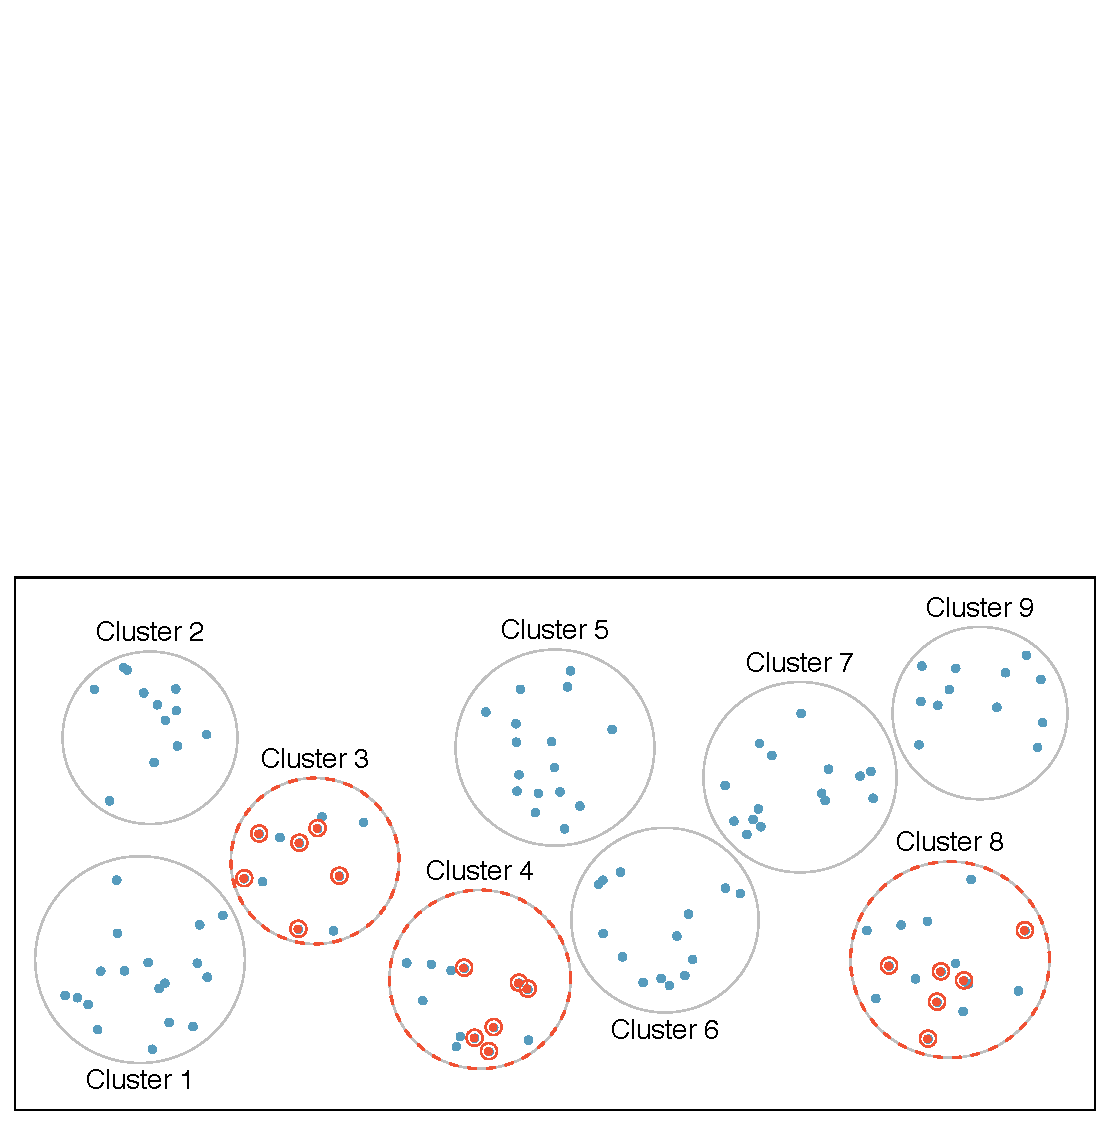
\includegraphics[width=0.9\textwidth]{1-3_sampling_principles_strategies/figures/sampling_methods/multistage}
\end{center}

\end{frame}

%%%%%%%%%%%%%%%%%%%%%%%%%%%%%%%%%%%%

\begin{frame}
\frametitle{練習問題}

\pq{ある市議会が、市の郊外地区で世帯調査を実施するよう要請した。
この地区は多くの異なるユニークな地域（大型住宅が多い地域、アパートだけの地域など）に分かれている。
次のどの方法が\emph{最も}効果的でないか？}

\begin{enumerate}[(a)]
\item 単純無作為抽出
\solnMult{クラスター抽出}
\item 層化抽出
\item ブロックサンプリング
\end{enumerate}

\end{frame}

%%%%%%%%%%%%%%%%%%%%%%%%%%%%%%%%%%%%
